%%%%%%%%%%%%%%%%%%%%%%%%%%%%%%%%%%%%%%%%%%%%%%%%%%%%%%%%%%%%%%%%%%%%%%%%%%%%%%%%
% PREÂMBULO
%%%%%%%%%%%%%%%%%%%%%%%%%%%%%%%%%%%%%%%%%%%%%%%%%%%%%%%%%%%%%%%%%%%%%%%%%%%%%%%%
\documentclass[a4paper, 11pt]{article}

% Pacotes de codificação e idioma
\usepackage[utf8]{inputenc}
\usepackage[T1]{fontenc}
\usepackage[brazil]{babel}

% Pacotes de formatação e conteúdo
\usepackage[margin=2.5cm]{geometry}
\usepackage{amsmath}
\usepackage{graphicx}
\usepackage{float}
\usepackage{hyperref}
\hypersetup{
    colorlinks=true,
    linkcolor=blue,
    filecolor=magenta,      
    urlcolor=cyan,
}

% Pacote para listagem de código
\usepackage{listings}
\usepackage{xcolor}

\definecolor{codegreen}{rgb}{0,0.6,0}
\definecolor{codegray}{rgb}{0.5,0.5,0.5}
\definecolor{codepurple}{rgb}{0.58,0,0.82}
\definecolor{backcolour}{rgb}{0.95,0.95,0.92}

\lstdefinestyle{pythonstyle}{
    backgroundcolor=\color{backcolour},   
    commentstyle=\color{codegreen},
    keywordstyle=\color{magenta},
    numberstyle=\tiny\color{codegray},
    stringstyle=\color{codepurple},
    basicstyle=\footnotesize\ttfamily,
    breakatwhitespace=false,         
    breaklines=true,                 
    captionpos=b,                    
    keepspaces=true,                 
    numbers=left,                    
    numbersep=5pt,                  
    showspaces=false,                
    showstringspaces=false,
    showtabs=false,                  
    tabsize=2
}
\lstset{style=pythonstyle}


% Informações do documento
\title{Estimação Recursiva de Parâmetros}
\author{Eduardo Henrique Basilio de Carvalho}
\date{\today}


%%%%%%%%%%%%%%%%%%%%%%%%%%%%%%%%%%%%%%%%%%%%%%%%%%%%%%%%%%%%%%%%%%%%%%%%%%%%%%%%
% DOCUMENTO
%%%%%%%%%%%%%%%%%%%%%%%%%%%%%%%%%%%%%%%%%%%%%%%%%%%%%%%%%%%%%%%%%%%%%%%%%%%%%%%%
\begin{document}

\maketitle

\section*{Introdução}

Este relatório detalha a implementação, comparação e análise de um conjunto de algoritmos de estimação recursiva de parâmetros. Os exercícios abordam desde a estimação de parâmetros em sistemas lineares com parâmetros constantes (LTI) até o rastreamento de parâmetros variantes no tempo e a aplicação dos métodos em dados experimentais de um sistema térmico. O objetivo principal é validar experimentalmente as propriedades teóricas dos estimadores, como convergência, viés e variância, e avaliar seu desempenho sob condições ideais e não ideais, como a presença de ruído com média não-nula ou ruído colorido.

\section*{Exercício 1: Fundamentos dos Estimadores Recursivos}
Neste exercício, foi investigado o desempenho de quatro famílias de estimadores recursivos na identificação de um sistema ARX de primeira ordem com parâmetros constantes.

\subsection*{1.a) Estimador Recursivo Não Polarizado}
\subsubsection*{Análise dos Resultados}
Os resultados dos histogramas mostram uma diferença marcante de desempenho entre os estimadores do tipo Gradiente e Gauss-Newton. O método de Gradiente, com um ganho fixo $\overline{K}$ bem ajustado, apresenta estimativas com um viés baixo (especialmente para $b_1$) e uma variância contida, resultando em uma distribuição concentrada em torno do valor verdadeiro. Em contraste, o método de Gauss-Newton, cuja atualização depende do termo $(\Psi_k^T \Psi_k)^{-1}$, exibe uma variância extremamente alta. Isso sugere uma sensibilidade numérica: quando o vetor de regressores $\Psi_k$ tem uma norma pequena, a inversão amplifica drasticamente o ruído, gerando estimativas espúrias (\textbf{outliers}) que deslocam a média e alargam a distribuição. A implicação prática é que, embora teoricamente robusto, o método de Gauss-Newton simplificado é numericamente instável sem uma normalização adequada, como a proposta na equação 13 do material de aula.

\begin{figure}[H]
    \centering
    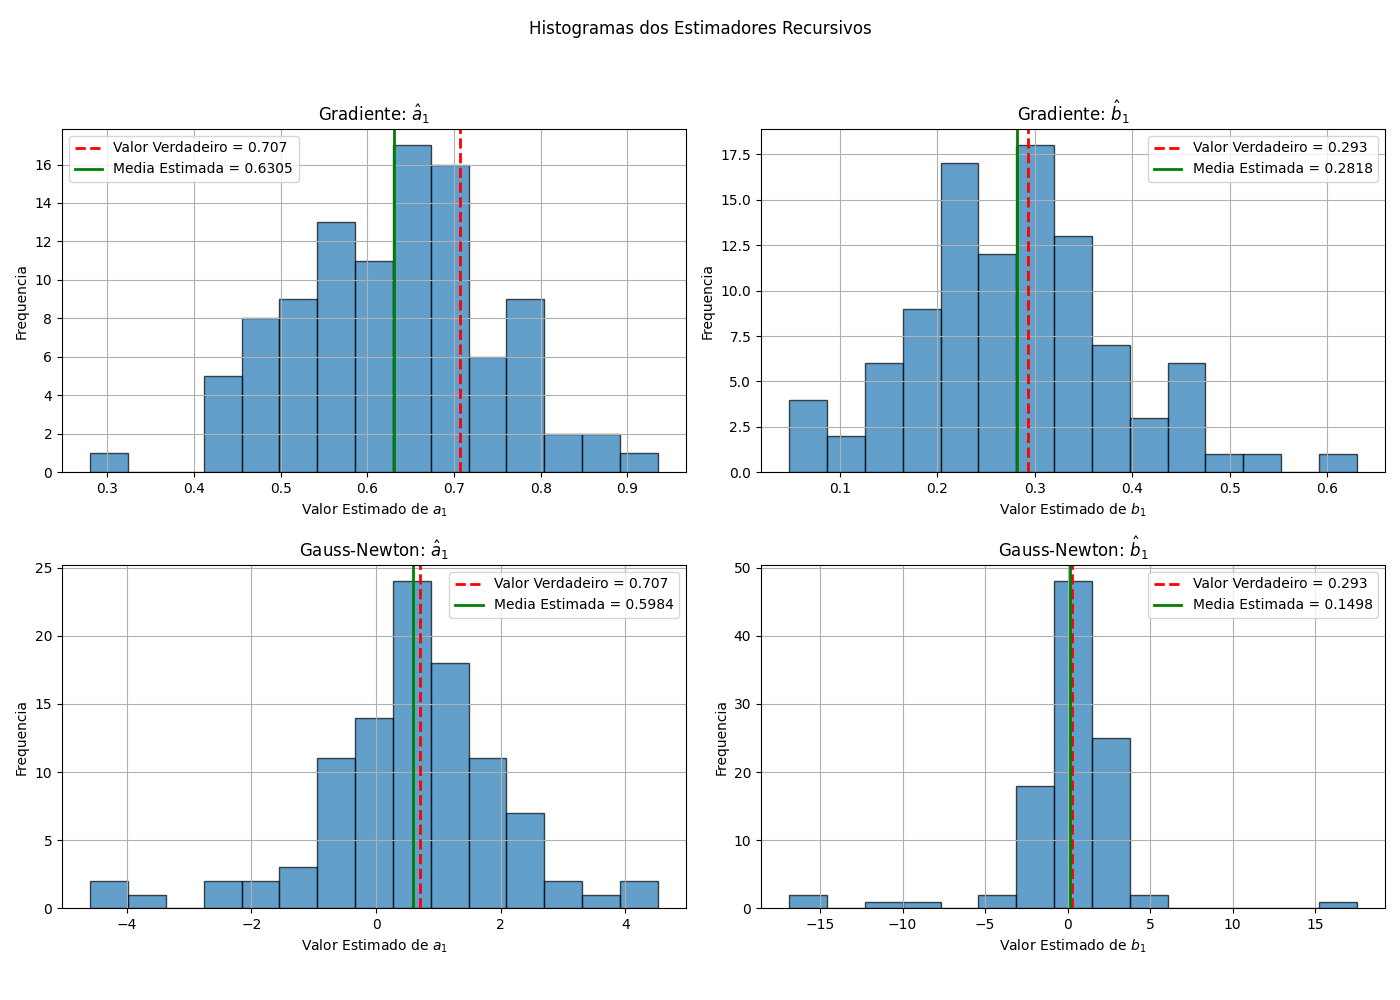
\includegraphics[width=\textwidth]{imagens/1a_histograma.png}
    \caption{Histogramas para os estimadores tipo Gradiente e Gauss-Newton.}
\end{figure}

\subsection*{1.b) Estimador de Aproximação Estocástica}
\subsubsection*{Análise dos Resultados}
A introdução do termo de decaimento $k^{-\alpha}$ nos ganhos, característico da aproximação estocástica, teve um efeito estabilizador notável. Para ambos os métodos, a variância foi drasticamente reduzida. Isso ocorre porque, à medida que $k$ aumenta, o ganho de atualização diminui, tornando o estimador menos suscetível ao ruído em amostras futuras, favorecendo a convergência. Para o método de Gauss-Newton, essa redução de ganho mitigou a instabilidade numérica, resultando em uma forte redução do viés. Contudo, para o método de Gradiente, o viés aumentou. Uma hipótese é que o ganho decai muito rapidamente, fazendo com que o algoritmo "congele" em uma estimativa sub-ótima antes de alcançar o valor verdadeiro, um clássico compromisso entre velocidade de convergência e precisão final.

\begin{figure}[H]
    \centering
    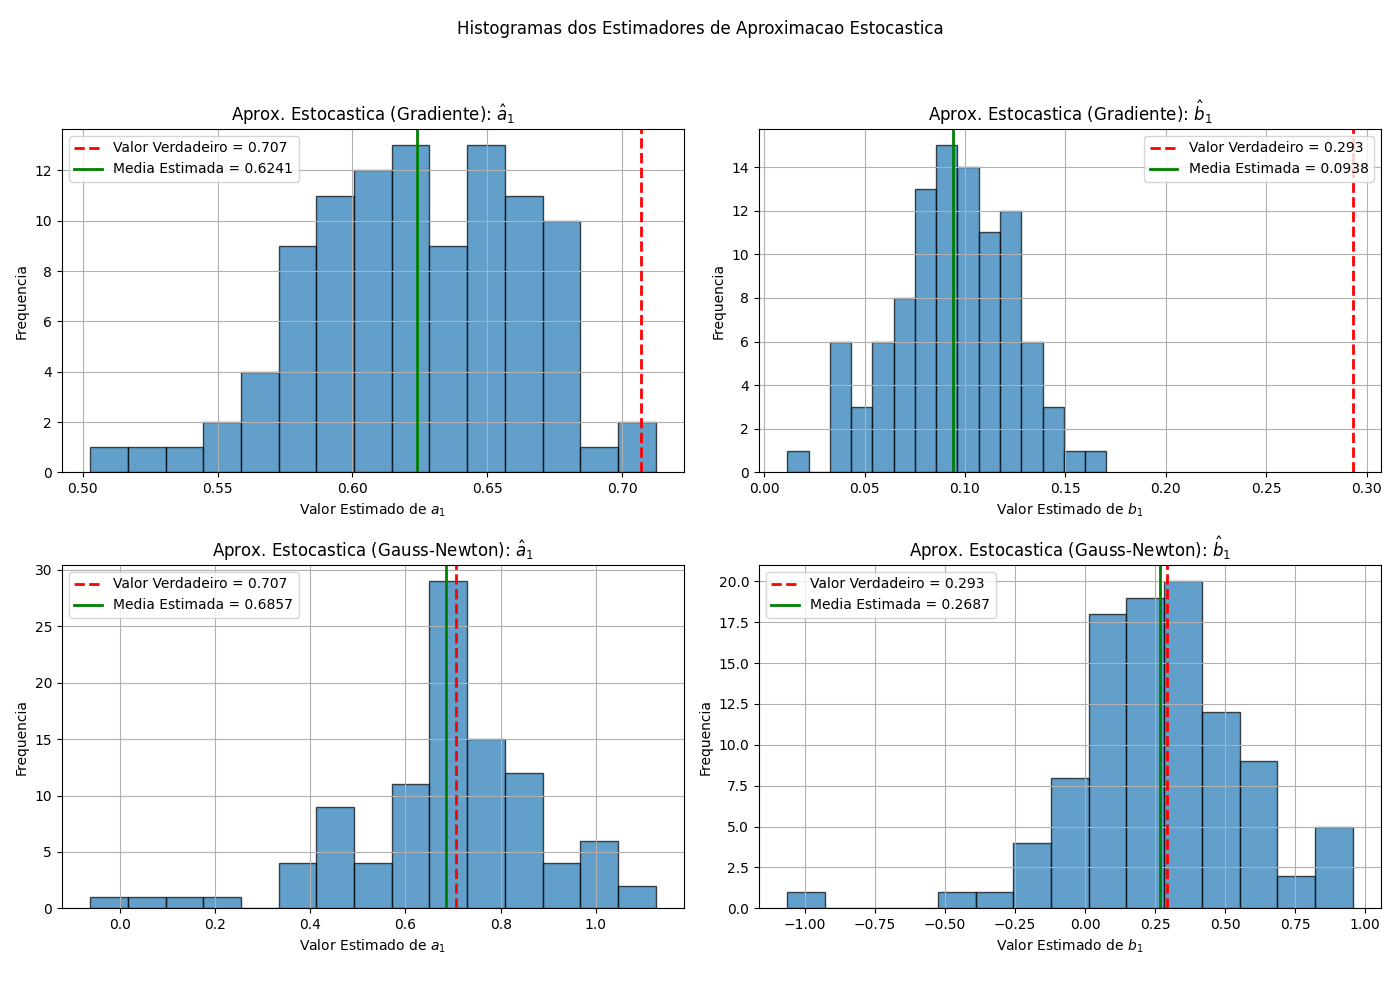
\includegraphics[width=\textwidth]{imagens/1b_histograma.png}
    \caption{Histogramas para os estimadores de aproximação estocástica.}
\end{figure}

\subsection*{1.c) Estimador de Mínima Covariância}
\subsubsection*{Análise dos Resultados}
O estimador de Mínima Covariância, que é uma formulação do Filtro de Kalman para estimação de parâmetros, apresentou um desempenho exemplar. Ao utilizar o conhecimento da covariância do ruído ($R$) e propagar a matriz de covariância da estimativa ($P_k$), o algoritmo calcula um ganho ótimo a cada passo. O resultado, como visto nos histogramas, é uma estimativa com viés desprezível e variância mínima entre os métodos testados. Isso valida a teoria de que, quando o modelo do sistema e as estatísticas do ruído são conhecidas, este estimador é ótimo no sentido de minimizar a variância do erro de estimação.

\begin{figure}[H]
    \centering
    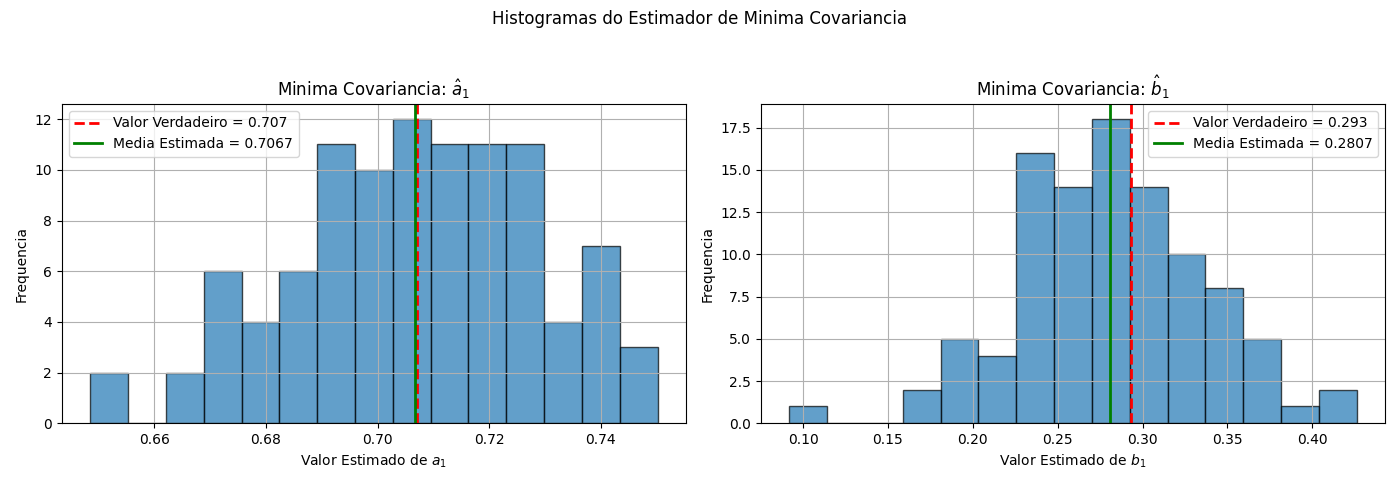
\includegraphics[width=\textwidth]{imagens/1c_histograma.png}
    \caption{Histogramas para o estimador de mínima covariância.}
\end{figure}

\subsection*{1.d) Mínimos Quadrados Recursivo (MQR)}
\subsubsection*{Análise dos Resultados}
O MQR demonstrou um desempenho praticamente idêntico ao do estimador de Mínima Covariância, com viés desprezível e variância muito baixa. A principal diferença teórica é que o MQR minimiza o somatório dos erros quadráticos, enquanto a Mínima Covariância minimiza a variância da estimativa final. Na prática, para ruído branco com média zero, os dois convergem para soluções muito semelhantes. A robustez e a eficiência do MQR, sem a necessidade de conhecer a covariância do ruído \textbf{a priori}, fazem dele um dos métodos mais populares e utilizados em aplicações práticas.

\begin{figure}[H]
    \centering
    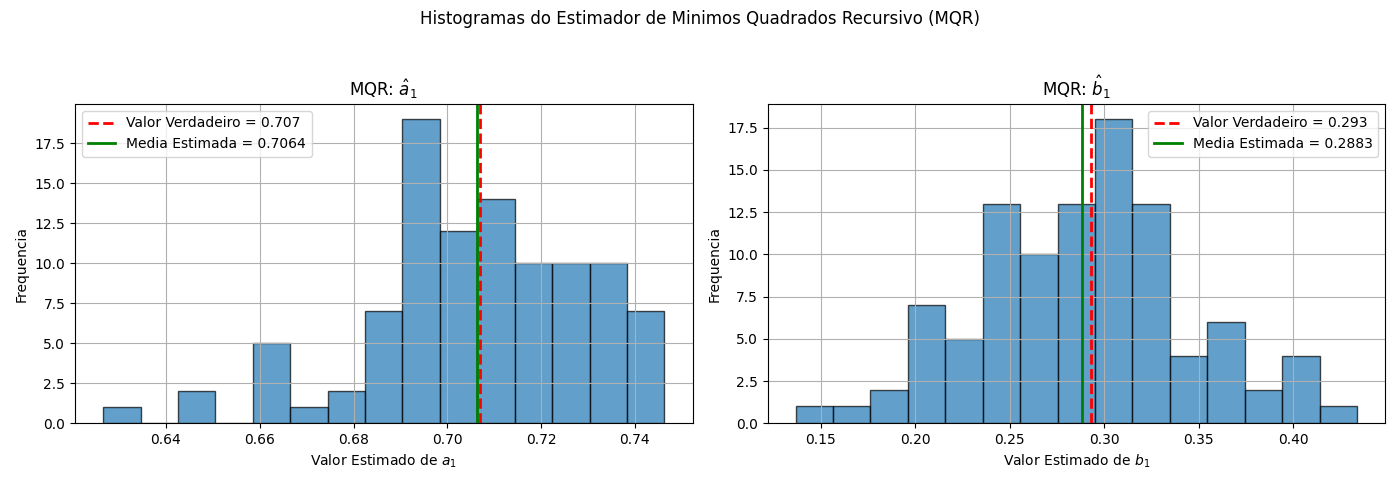
\includegraphics[width=\textwidth]{imagens/1d_histograma.png}
    \caption{Histogramas para o estimador MQR.}
\end{figure}

\subsection*{1.e) Comparação Geral e Impacto de N}
\subsubsection*{Análise dos Resultados}
A análise assintótica confirma as propriedades teóricas dos estimadores. Para os métodos consistentes (MQR, Mínima Covariância, e as variantes de Gradiente), o viés e a variância tendem a diminuir à medida que mais amostras (N) são utilizadas, pois mais informação é agregada para refinar a estimativa. Notavelmente, MQR e Mínima Covariância exibem uma taxa de convergência superior, com a variância caindo de forma mais acentuada. O comportamento da variância do método de Gradiente (que aumenta e depois estabiliza) é interessante; uma hipótese é que o ganho fixo $\overline{K}$ continua a injetar uma quantidade constante de incerteza a cada passo (termo $K_k R K_k^T$ na equação 16), o que limita a redução da variância final, diferentemente dos métodos cujo ganho diminui com o tempo. O comportamento errático de Gauss-Newton reforça sua instabilidade.

\begin{figure}[H]
    \centering
    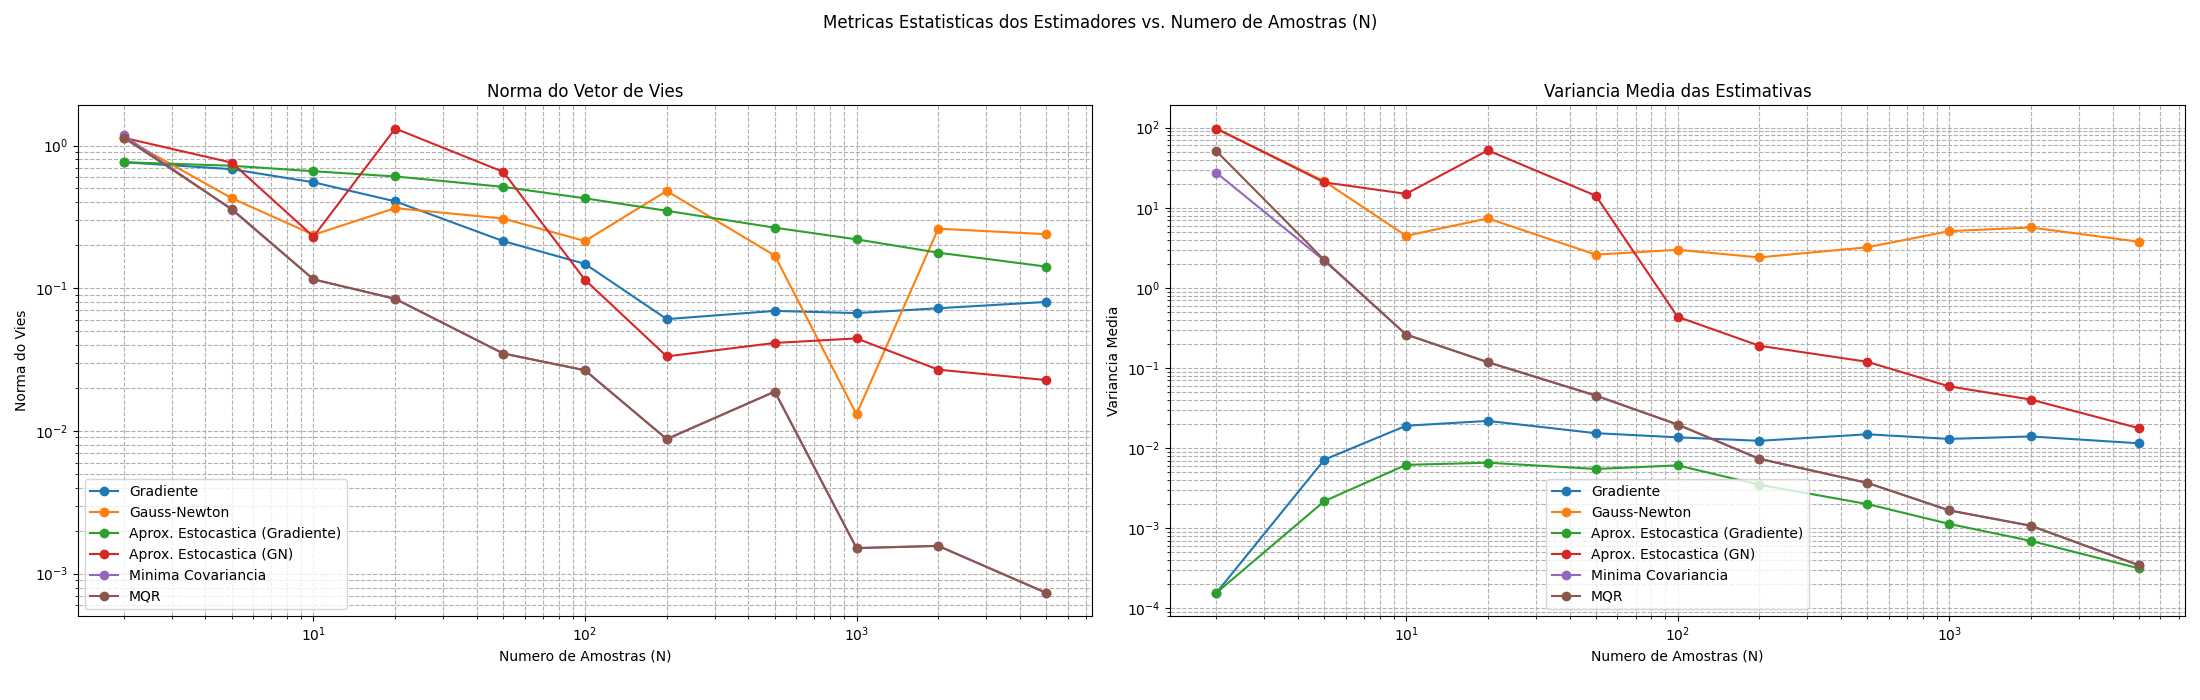
\includegraphics[width=\textwidth]{imagens/1e_estatisticas_vs_N.png}
    \caption{Evolução do viés e variância em função do número de amostras (N).}
\end{figure}

\subsection*{1.f) Trajetória dos Parâmetros}
\subsubsection*{Análise dos Resultados}
A evolução temporal das estimativas para uma única realização de ruído ilustra a dinâmica de cada algoritmo. O MQR e a Mínima Covariância convergem suave e rapidamente para os valores verdadeiros, demonstrando sua eficiência. A Aproximação Estocástica do Gradiente mostra uma convergência muito mais lenta, porém estável e com baixo ruído no estado estacionário. Em contraste, o Gradiente com ganho fixo converge rápido, mas a estimativa permanece ruidosa, oscilando em torno do valor real. Os métodos baseados em Gauss-Newton mostram picos de alta amplitude, evidenciando a instabilidade numérica já discutida. A trajetória de MQR e Mínima Covariância é o comportamento desejado para a identificação de sistemas LTI.

\begin{figure}[H]
    \centering
    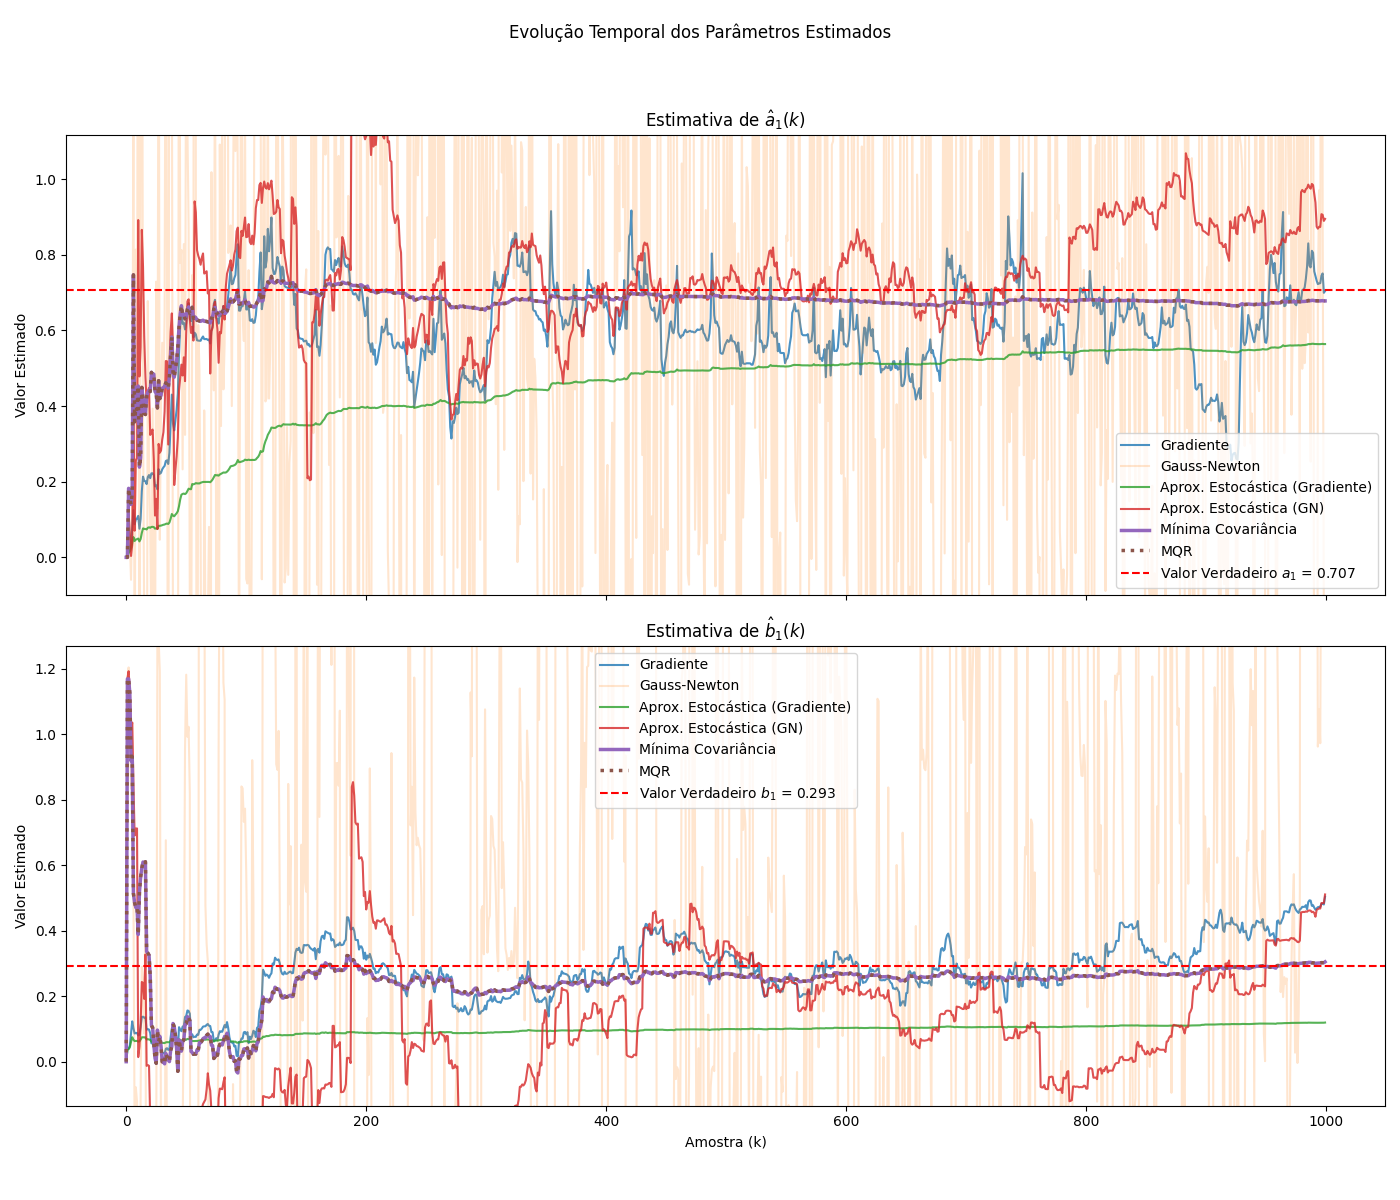
\includegraphics[width=\textwidth]{imagens/1f_trajetoria_parametros.png}
    \caption{Evolução temporal das estimativas de parâmetros para cada método.}
\end{figure}

\newpage
\section*{Exercício 2: Parâmetros Variantes no Tempo}
Este exercício avaliou a capacidade de rastrear parâmetros que mudam com o tempo.

\subsection*{2.a) Efeito do Fator de Esquecimento ($\lambda$)}
\subsubsection*{Análise dos Resultados}
O fator de esquecimento $\lambda$ no MQR-FF ajusta a "memória" do estimador. Valores de $\lambda$ próximos de 1 (e.g., 0.999) atribuem um peso maior aos dados passados, resultando em uma estimativa suave, mas com um atraso significativo no rastreamento (viés dinâmico). Valores menores de $\lambda$ (e.g., 0.9) "esquecem" o passado rapidamente, tornando o estimador mais ágil para seguir as variações, porém muito mais sensível ao ruído. O valor $\lambda=0.95$ representa um bom compromisso, conseguindo acompanhar a tendência dos parâmetros reais sem amplificar excessivamente o ruído. A escolha de $\lambda$ é, portanto, um compromisso fundamental entre a capacidade de rastreamento e a rejeição a ruído.

\begin{figure}[H]
    \centering
    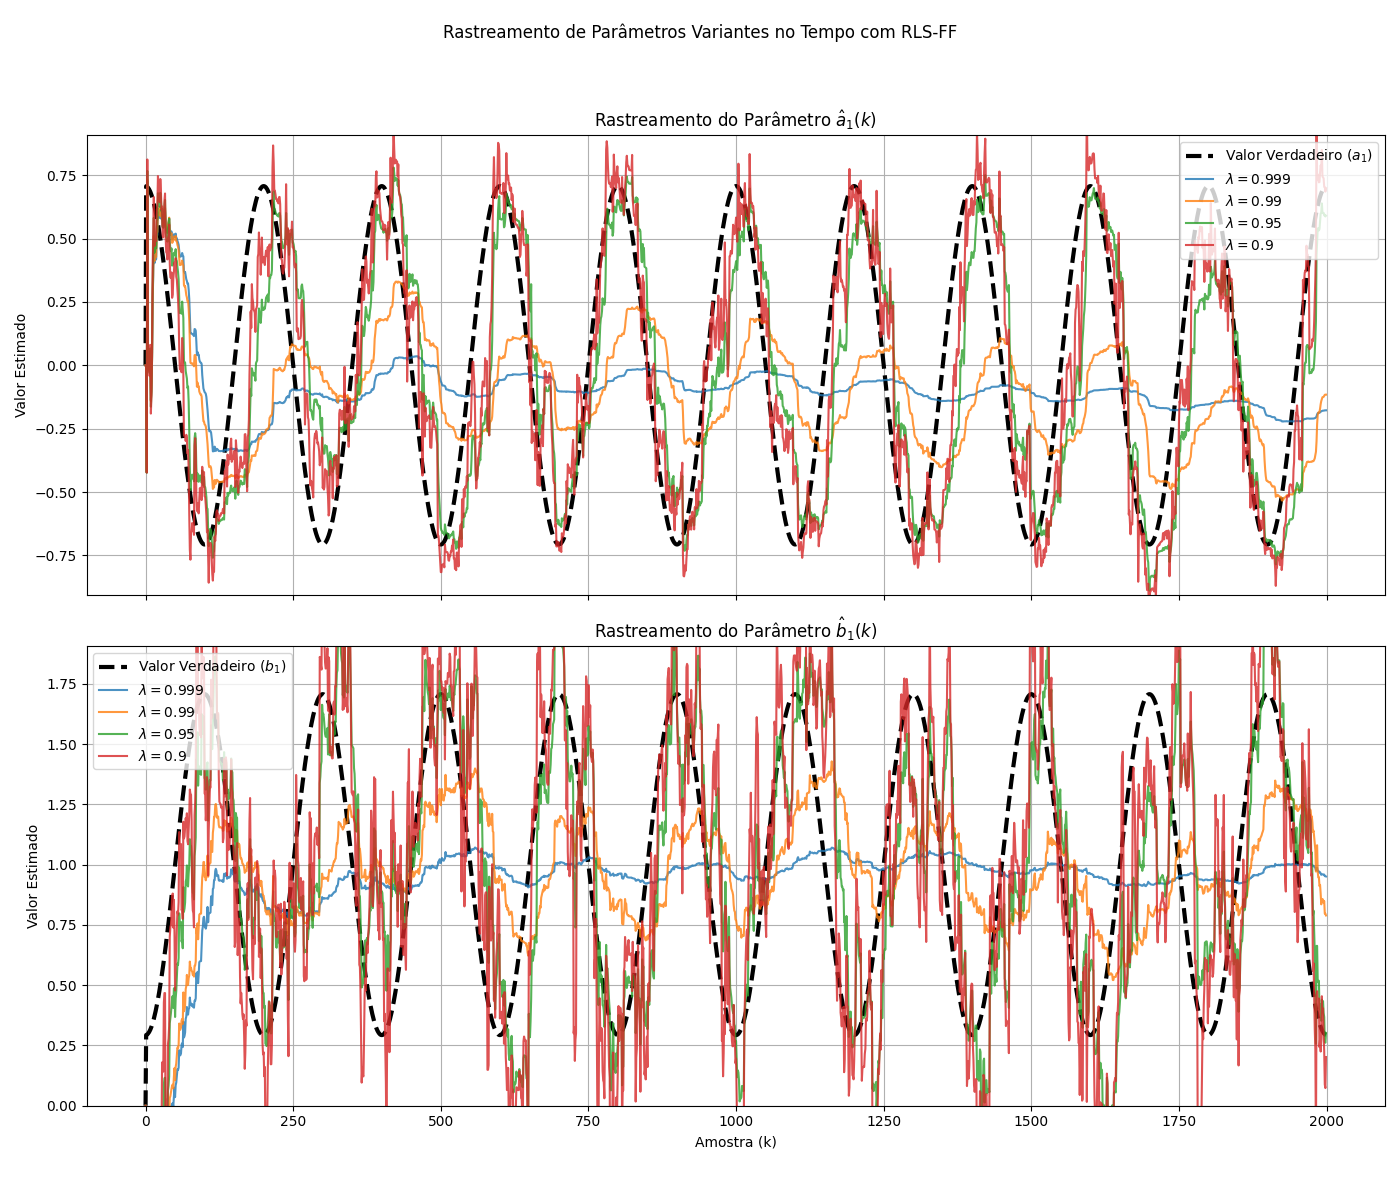
\includegraphics[width=\textwidth]{imagens/2a_rastreamento_lambda.png}
    \caption{Rastreamento de parâmetros variantes no tempo para diferentes valores de $\lambda$.}
\end{figure}

\subsection*{2.b) Efeito da Persistência de Excitação}
\subsubsection*{Análise dos Resultados}
A persistência de excitação é fundamental para a estimação de parâmetros, pois garante que o sistema seja "sondado" em diferentes direções, fornecendo informação suficiente para identificar todos os parâmetros. Ao manter a entrada constante por períodos mais longos (\textbf{hold}), a informação contida no vetor de regressores $\Psi_k$ torna-se pobre e, em alguns instantes, a matriz $\Psi_k^T \Psi_k$ pode se tornar mal condicionada. Os resultados mostram claramente a degradação do desempenho: quanto maior o período de \textbf{hold}, maior o atraso e o ruído nas estimativas. Isso ocorre porque o estimador não recebe "informação nova" suficiente para atualizar os parâmetros corretamente, fazendo com que a matriz de covariância $P_k$ cresça e o rastreamento se deteriore.

\begin{figure}[H]
    \centering
    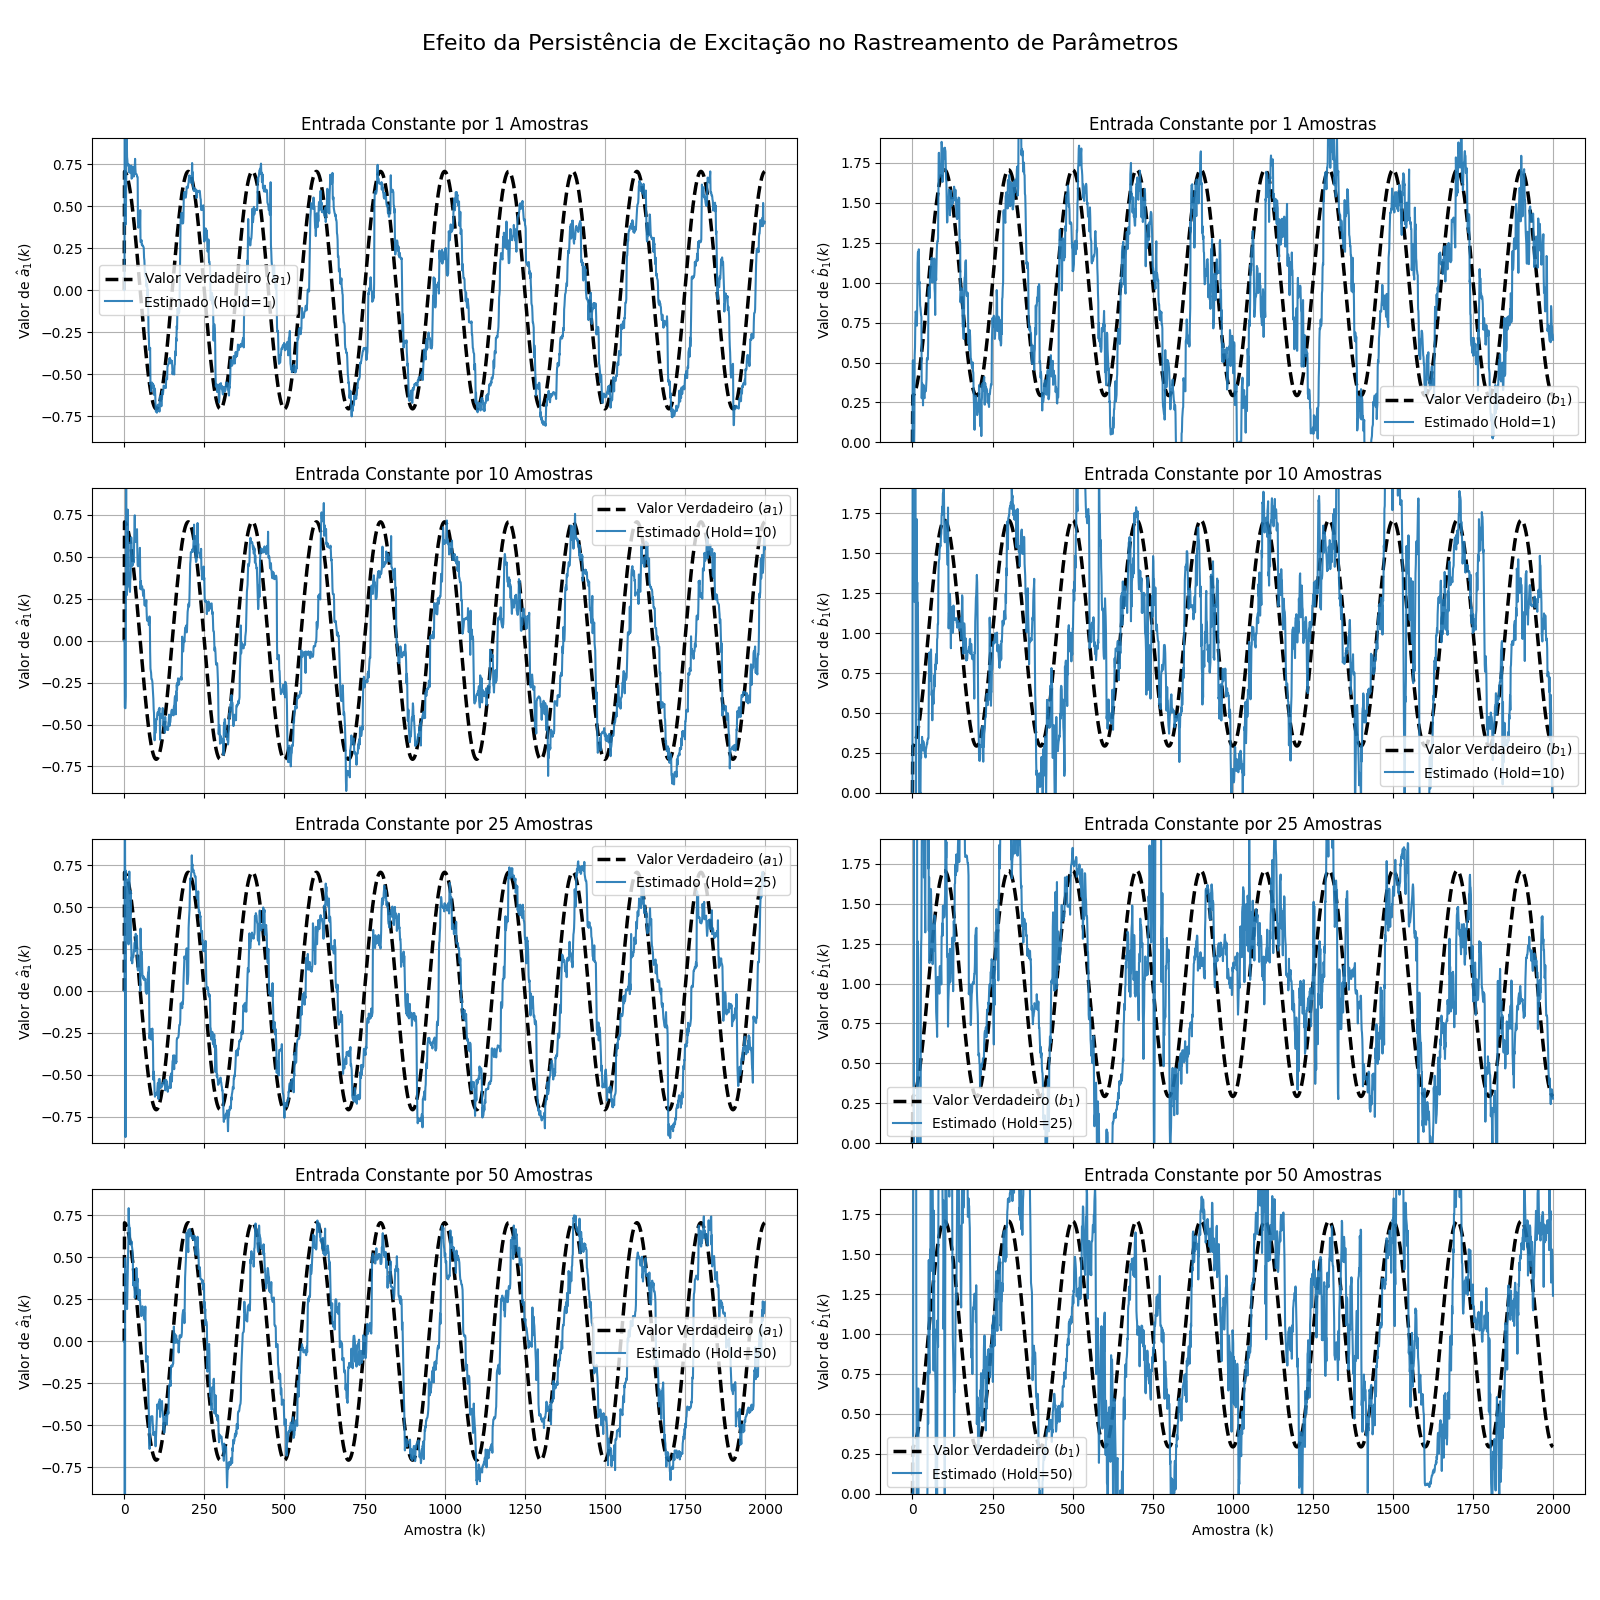
\includegraphics[width=\textwidth]{imagens/2b_persistencia_excitacao.png}
    \caption{Efeito da persistência de excitação na qualidade do rastreamento.}
\end{figure}

\newpage
\section*{Exercício 3: Condições Não Ideais}
Este exercício testou a robustez dos estimadores quando as premissas sobre o ruído são violadas.

\subsection*{3.a) Ruído com Média Não-Nula}
\subsubsection*{Análise dos Resultados}
Todos os estimadores implementados partem da premissa de que o ruído $\eta(k)$ tem média zero. Quando essa premissa é violada, o termo de ruído se comporta como um \textbf{offset} persistente, que é erroneamente incorporado na estimação dos parâmetros. Como resultado, os histogramas mostram que a média das estimativas de $a_1$ é significativamente deslocada, introduzindo um viés que não desaparece mesmo com muitas amostras. Isso demonstra uma limitação fundamental desses estimadores: eles não conseguem distinguir entre a dinâmica do processo e um distúrbio constante na saída. Para resolver isso, seria necessário aumentar o modelo, por exemplo, estimando um termo de \textbf{offset} adicional.

\begin{figure}[H]
    \centering
    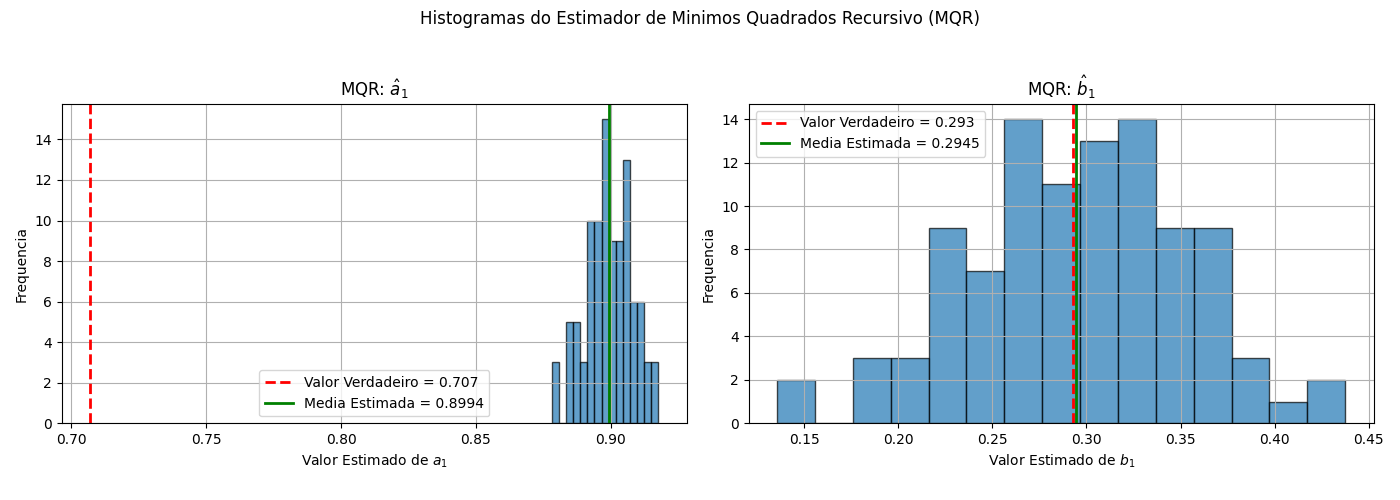
\includegraphics[width=0.8\textwidth]{imagens/3a_1d_histograma.png}
    \caption{Efeito da média não-nula no MQR para parâmetros constantes.}
\end{figure}

\subsection*{3.b) Ruído Colorido}
\subsubsection*{Análise dos Resultados}
O ruído colorido, que possui correlação temporal, viola outra premissa central do MQR: a de que o erro de predição em um instante não está correlacionado com os regressores passados. Quando essa correlação existe, como no caso do ruído colorido, o MQR produz estimativas enviesadas. Os histogramas mostram claramente que a média das estimativas de $a_1$ está deslocada do valor verdadeiro. O viés é persistente e não é corrigido com o aumento do número de amostras. Para lidar com ruído colorido, seriam necessárias técnicas mais avançadas, como o método das Variáveis Instrumentais (IV) ou o Mínimos Quadrados Estendido (Extended Least Squares - ELS), que modelam explicitamente a dinâmica do ruído.

\begin{figure}[H]
    \centering
    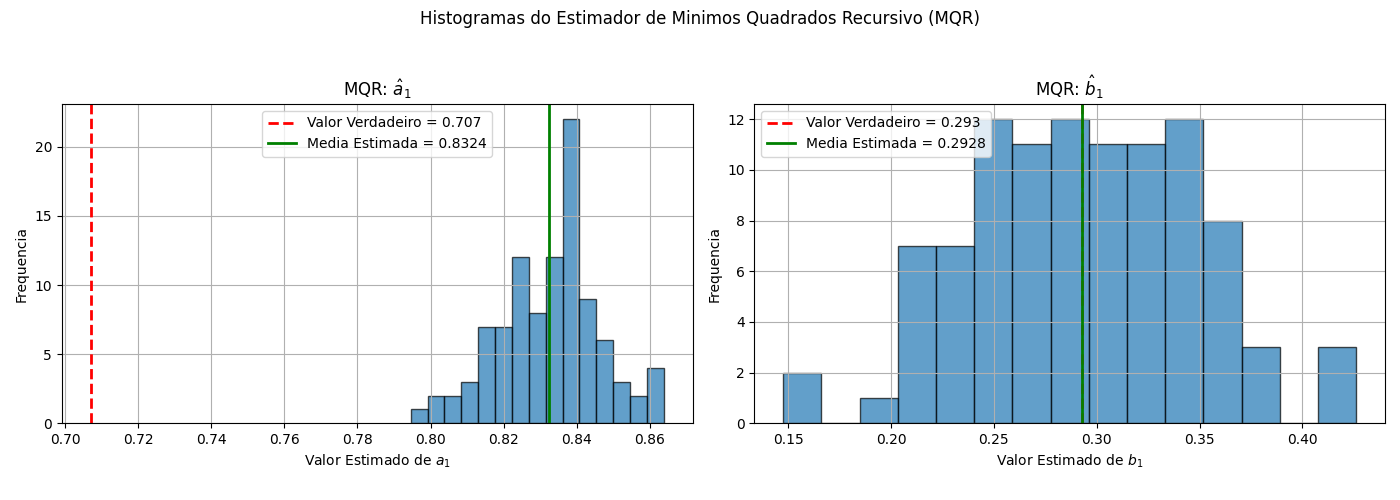
\includegraphics[width=0.8\textwidth]{imagens/3b_1d_histograma.png}
    \caption{Efeito do ruído colorido no MQR para parâmetros constantes.}
\end{figure}

\newpage
\section*{Exercício 4: Aplicação em Dados Reais}
Neste exercício, os métodos foram aplicados para identificar um modelo para um sistema térmico real.

\subsection*{4.a) Pré-processamento dos Dados}
\subsubsection*{Análise dos Resultados}
O pré-processamento dos dados foi uma etapa fundamental. Sistemas térmicos possuem dinâmicas lentas, tornando-os suscetíveis a superamostragem. A remoção dos transitórios inicial e final garantiu que apenas dados em regime fossem utilizados para a identificação. A remoção da média focou o modelo na dinâmica de variação em torno do ponto de operação. Finalmente, a decimação reduziu a carga computacional e a correlação entre amostras consecutivas, o que é benéfico para os algoritmos de estimação. Os gráficos mostram a transformação de um sinal longo e com variações lentas em um sinal mais curto e adequado para a modelagem ARX.

\begin{figure}[H]
    \centering
    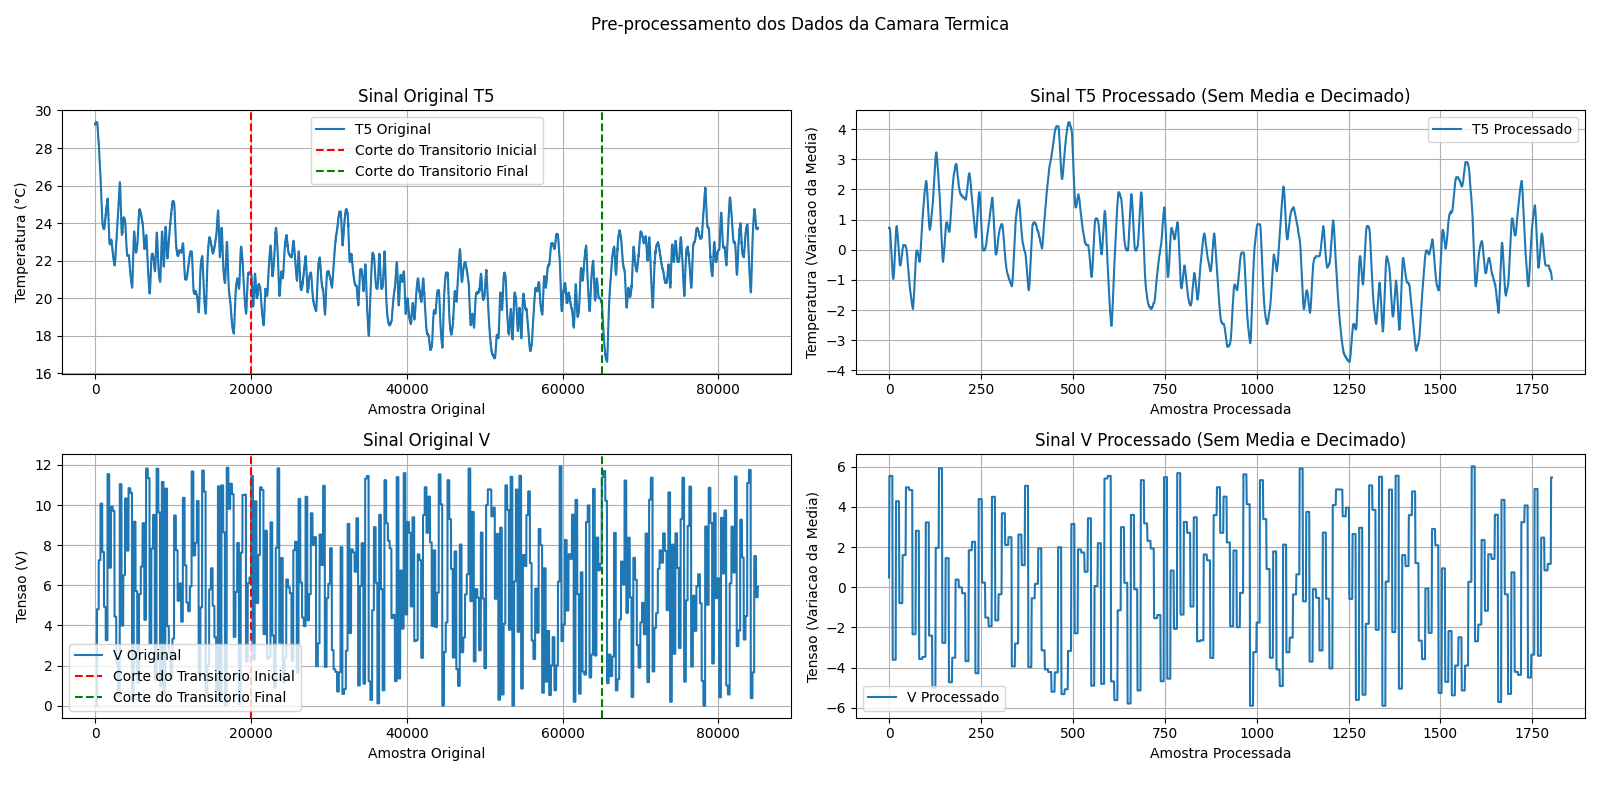
\includegraphics[width=\textwidth]{imagens/4a_processamento_dados.png}
    \caption{Comparação dos sinais originais e processados.}
\end{figure}

\subsection*{4.b) Estimação com MQR Padrão}
\subsubsection*{Análise dos Resultados}
O MQR Padrão, ao ser aplicado aos dados da câmara térmica, produziu estimativas de parâmetros que convergem e se estabilizam. Isso sugere que um modelo LTI (Linear Time-Invariant) de ordem 4 é uma aproximação razoável para a dinâmica do sistema em torno do ponto de operação. A estabilização dos parâmetros indica que o algoritmo encontrou um conjunto de valores que minimiza o erro quadrático ao longo de todo o conjunto de dados.

\begin{figure}[H]
    \centering
    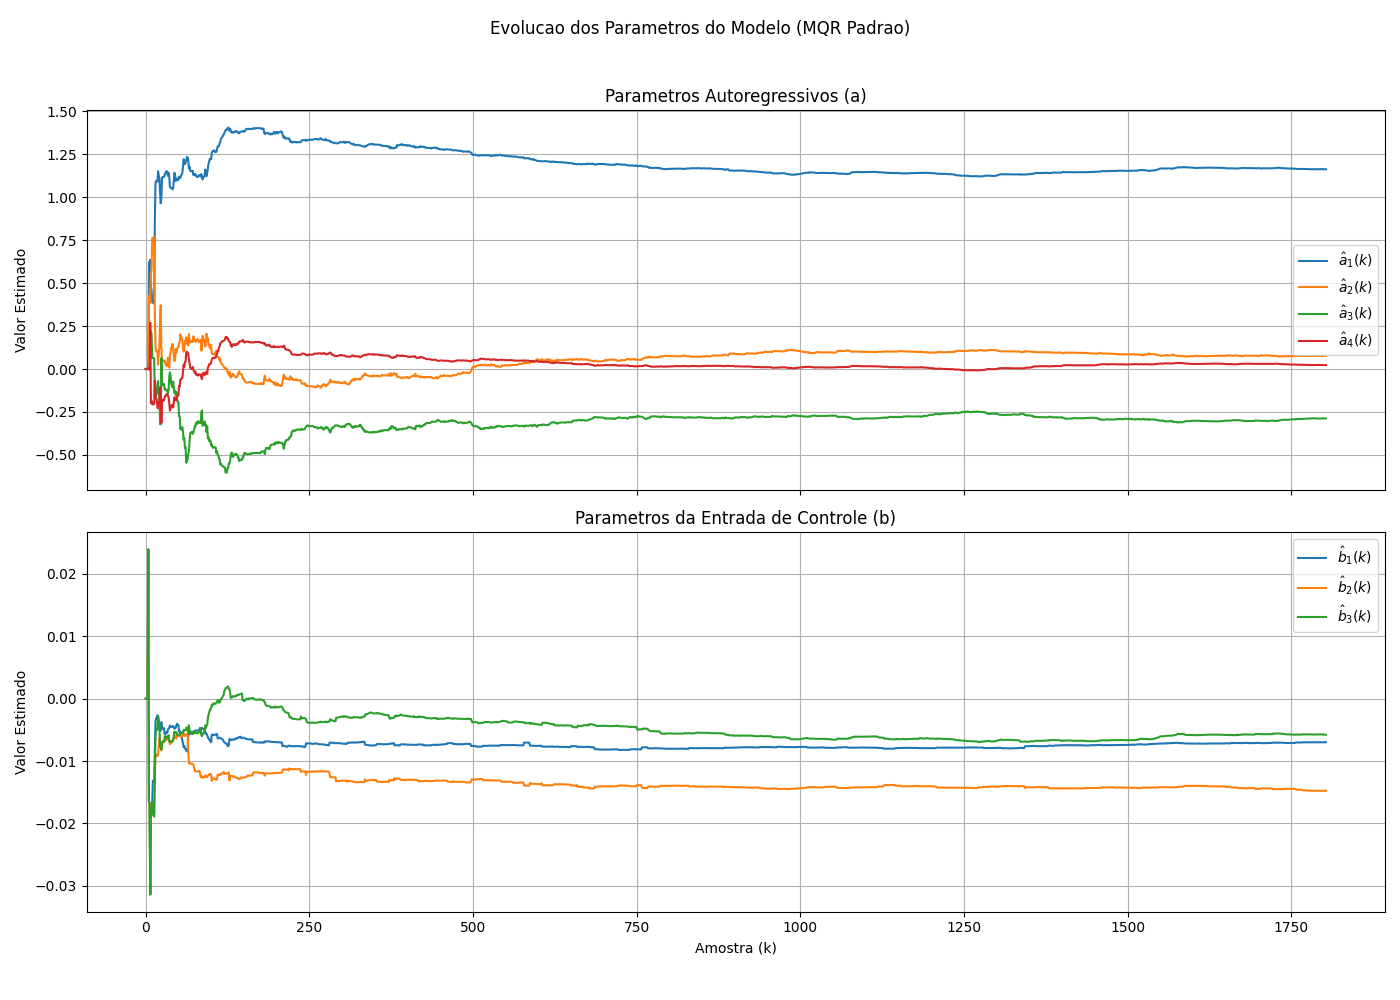
\includegraphics[width=\textwidth]{imagens/4b_parametros_mqr.png}
    \caption{Evolução dos parâmetros do modelo com MQR Padrão.}
\end{figure}

\subsection*{4.c) Estimador de Espaço de Estados (Filtro de Kalman)}
\subsubsection*{Análise dos Resultados}
O Filtro de Kalman, configurado para estimar parâmetros, permite modelar a incerteza não apenas na medição (R), mas também nos próprios parâmetros (Q). Ao usar uma matriz Q não nula, assume-se que os parâmetros podem variar ao longo do tempo (modelo de passeio aleatório). O resultado são trajetórias de parâmetros mais suaves em comparação com o MQR-FF, pois o filtro otimamente equilibra a informação nova com a predição do estado anterior. As variações suaves nos parâmetros de 'a' podem estar capturando a dinâmica real de como a eficiência de troca térmica muda com a temperatura ambiente, que, como mencionado no enunciado, variou durante o experimento.

\begin{figure}[H]
    \centering
    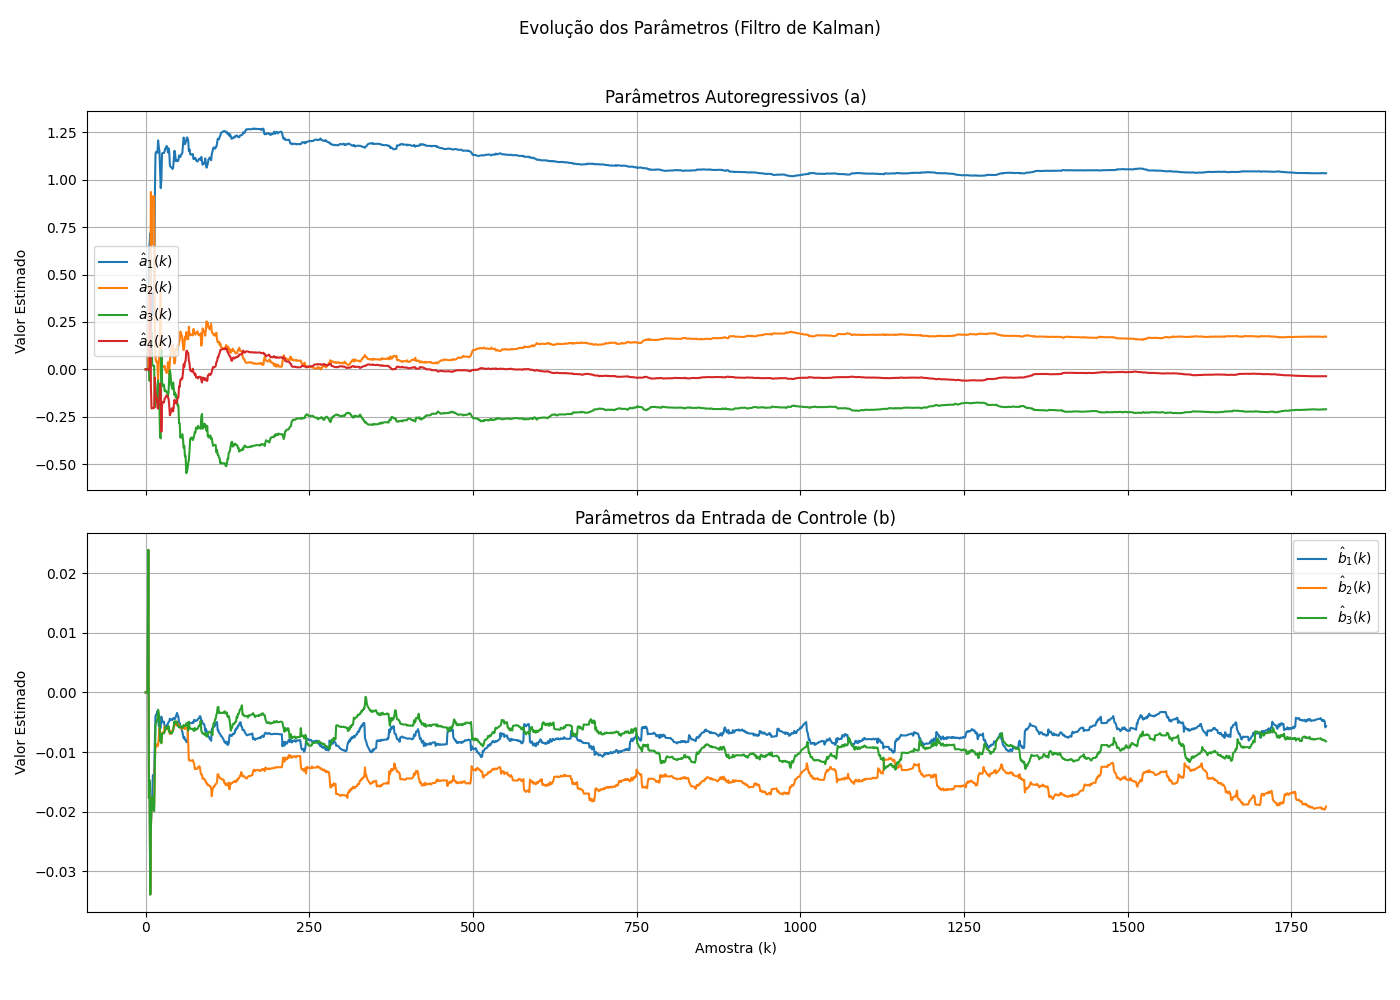
\includegraphics[width=\textwidth]{imagens/4c_parametros_kalman_filter.png}
    \caption{Evolução dos parâmetros do modelo com Filtro de Kalman.}
\end{figure}

\subsection*{4.d) Estimação com MQR com Fator de Esquecimento}
\subsubsection*{Análise dos Resultados}
A utilização do MQR com Fator de Esquecimento (MQR-FF) assume explicitamente que os parâmetros do sistema não são constantes. O valor de $\lambda=0.995$ confere ao estimador uma memória longa, permitindo que ele se adapte a variações lentas, o que é apropriado para um sistema térmico. As trajetórias dos parâmetros, embora ainda ruidosas, mostram variações consistentes que não estão presentes no MQR padrão. Uma hipótese plausível é que essas variações estão rastreando mudanças reais na dinâmica do sistema, causadas por fatores não modelados, como a variação da temperatura ambiente ao longo do longo período de coleta de dados. Isso demonstra a superioridade de um modelo adaptativo para sistemas que operam por longos períodos em condições variáveis.

\begin{figure}[H]
    \centering
    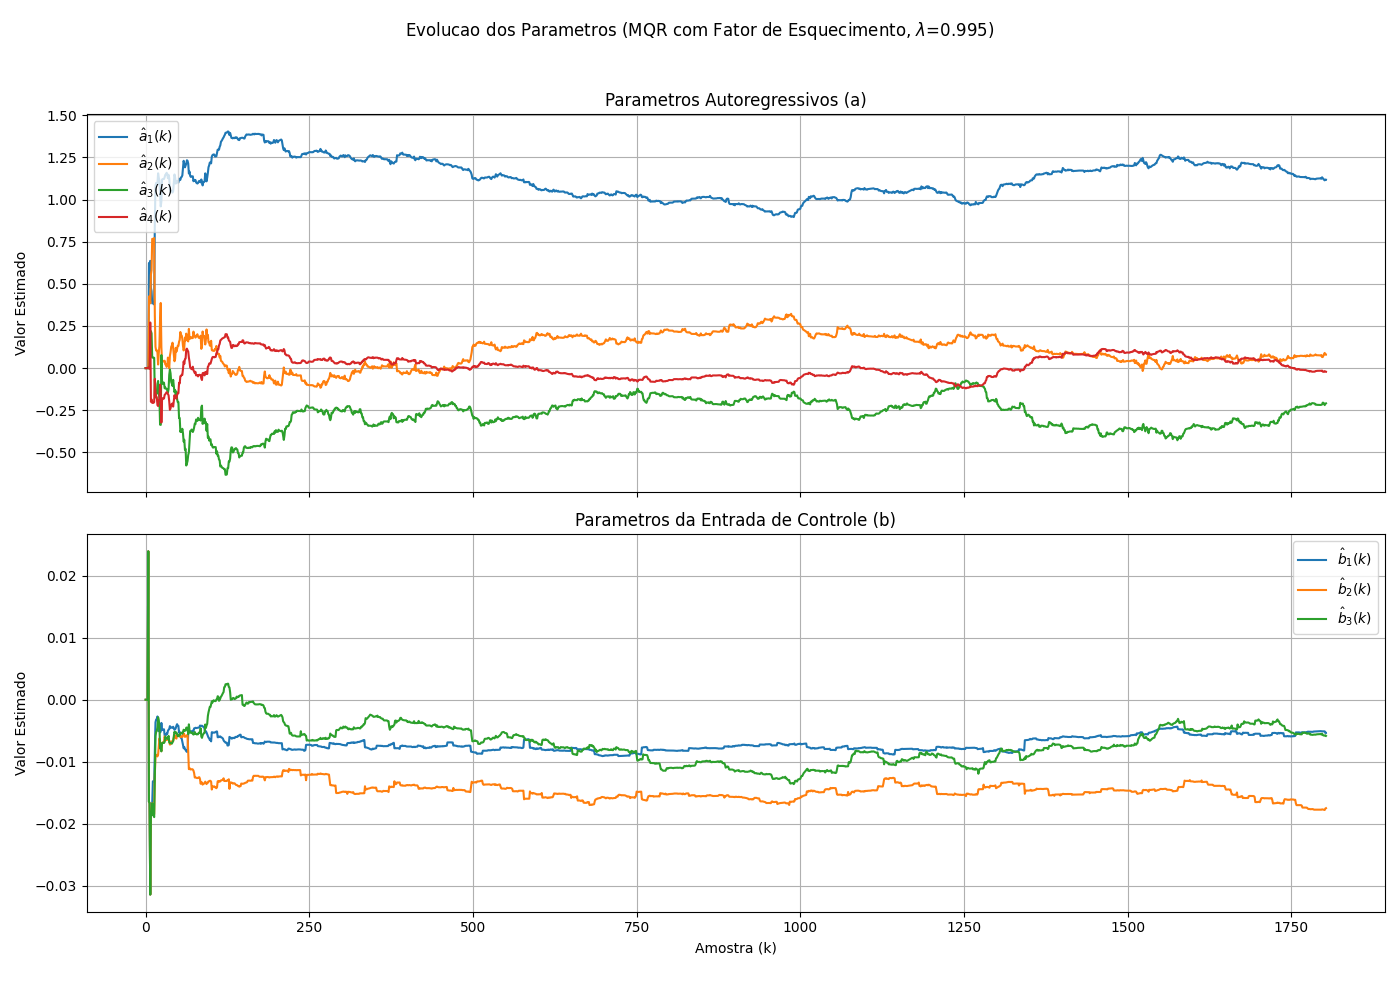
\includegraphics[width=\textwidth]{imagens/4d_parametros_mqr_ff.png}
    \caption{Evolução dos parâmetros com MQR com Fator de Esquecimento ($\lambda=0.995$).}
\end{figure}

\newpage
\section*{Conclusão Geral}
Este estudo permitiu uma análise prática e comparativa de diversos estimadores recursivos. Para sistemas com parâmetros constantes e ruído branco, os estimadores de Mínima Covariância e MQR mostraram-se superiores, com rápida convergência e baixa variância. Para parâmetros variantes no tempo, o MQR com fator de esquecimento (MQR-FF) demonstrou ser eficaz, embora a escolha do fator $\lambda$ seja um compromisso crucial entre agilidade e robustez ao ruído. Os exercícios também destacaram a importância das condições ideais: a presença de ruído com média não-nula ou colorido degrada o desempenho dos estimadores, introduzindo viés. Finalmente, a aplicação a dados reais de um sistema térmico mostrou que métodos adaptativos, como o Filtro de Kalman ou o MQR-FF, podem ser mais adequados para capturar a dinâmica de sistemas cujos parâmetros variam lentamente com o tempo devido a influências externas.

\end{document}